%--------------------------------------
% ICPHILCOMP 25 LaTeX Beamer template
% Based on CleanEasy by Jose Paulo Marchezi
% https://github.com/zemarchezi/CleanEasy_BeamerTheme
% This template is distributed under the CC BY-NC 4.0 License:
% https://creativecommons.org/licenses/by-nc/4.0/
%
% ICPHILCOMP, Philosophy of Computing and Filosofía de la Computación
% logos and trademarks property of the Philosophy of Computing Research Group. 
% Agile Design Studio is an AgileEngine trademark.
%--------------------------------------

% This is the tex source file where you should put your presentation content
% To modify the title, list of authors, institutions, etc. please refer to the
% "configs/title_page.tex"

% PACKAGES
\documentclass[aspectratio=169,xcolor=dvipsnames]{beamer}
\makeatletter
\def\input@path{{theme/}}
\makeatother
\usetheme{ICPHILCOMP25}
\usepackage{fix-cm}
\usepackage{amsmath}
\usepackage{mathtools}
\usepackage{listings}
\usepackage{xcolor}
\usepackage{hyperref}
\usepackage{graphicx}
\usepackage{booktabs}
\usepackage{tikz}
\usetikzlibrary{positioning, shapes, arrows, calc, decorations.pathreplacing, arrows.meta, backgrounds, patterns, overlay-beamer-styles}
\usepackage{etoolbox}
\usepackage{animate}
\usepackage{ dsfont }

%  LAYOUT CONFIGURATION
\input{configs/configs}
\title[Causalidad en Redes Neuronales]{¿Relaciones Causales en Redes Neuronales o Inferencias Inductivas?}

\author[Laura Dimayuga]{Laura Itzel Rodríguez Dimayuga\inst{1}}

\institute[UNAM]{\inst{1}%
  Facultad de Ciencias \\
  UNAM
}

\date{Febrero, 2026}
% Define positions for logos on title page
\titlegraphic{
  \begin{tikzpicture}[remember picture, overlay]
    % Here you can add a custom logo saved in the /speaker_resources directory:
    % Make sure to use a monochromatic white version of your institution.
    \node[anchor=north east, xshift=-1cm, yshift=-4cm] at (current page.north east) {
      
\includegraphics[height=1.5cm]{speaker_resources/philcomp_logo_white.png}
    };
  \end{tikzpicture}
}



% CONTENT
\begin{document}
\begin{frame}[plain]
  \titlepage
\end{frame}

\begin{frame}[plain]{Contents}
  \tableofcontents
\end{frame}

\section{Introducción}
\subsection{Pregunta Central}
  \begin{frame}{Pregunta Central}
    \begin{block}{Pregunta Central}
      ¿Hemos logrado substraer relaciones causales en los modelos más recientes de redes neuronales o LLMs?
      ¿Qué nos demuestra la posibilidad de inferir causalidades que se observan en nuestra realidad observable a partir de estos modelos?
    \end{block}
    
    \begin{exampleblock}{Importancia de la pregunta}
      No solo existe una amplia gama de toma decisiones basadas en el resultado de estos modelos, existes diversos programas enfocados en usar modelos para encontrar descubrimientos científicos con técnicas de aprendizaje automático (ej. \cite{hey2009fourth, wang2023scientific,ioannidis20245th, bianchini2020deep}). 
      Si las inferencias causales constituyen nuestra manera de hacer conocimiento, tenemos que demostrar que dichos modelos son capaces de sustraerlas. 
    \end{exampleblock}
  \end{frame}
\subsection{Motivaciones Epistémicas}
\begin{frame}{Motivaciones Epistémicas}
  ``This becomes a critical issue because science represents the set of tools humanity uses
for exploring and understanding ourselves, our universe, and our place in the web of
life here on Earth.We need to be able to trust our tools to help us solve problems in
the biosphere without generating side effects worse then the problems, themselves."(Judith Rosen, \cite{rosen2012anticipatory})
\end{frame}
\begin{frame}{Explicabilidad}
  La causalidad es uno de las cualidades que buscamos para intentar mejorar la explicabilidad de los modelos de aprendizaje profundo. Resaltado por \cite{doshi2017towards} buscamos lo siguiente: 
  \begin{itemize}
    \item \textbf{Equidad}: garantizar que las predicciones sean imparciales y no discriminen, de forma implícita o explícita, a grupos subrepresentados.
    \item \textbf{Privacidad}: garantizar que la información sensible en los datos esté protegida.
    \item \textbf{Confiabilidad o Robustez}: garantizar que pequeños cambios en la entrada no provoquen grandes cambios en la predicción.
    \item \textbf{Causalidad}: asegurar que solo se identifiquen relaciones causales.
    \item \textbf{Confianza}: para las personas es más fácil confiar en un sistema que explica sus decisiones que en una caja negra.
  \end{itemize}
\end{frame}
\begin{frame}{Relacion de Modelado}
  \begin{enumerate}
    \item Las relaciones existen en el mundo real
    \item Tales relaciones pueden ser descubiertas por la mente. Este descubrimiento no es directo, como el de las cualidades, sino que se imputa a la realidad desde el constructo mental.
    \item Diremos que una cualidad de un NS es observable cuando tal cualidad sea perceptible. Diremos que una relación producible entre dos observables es un \textbf{vínculo} (linkage). \cite{soto-astorga2025codificaciones}
  \end{enumerate}
  \begin{figure}
    \centering
    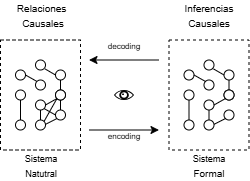
\includegraphics[height=0.3\textheight]{assets/tesis-model-relationship.png}
    \caption{Relación de modelado entre la realidad, los modelos y las inferencias causales.}
  \end{figure}
\end{frame}
\subsection{Antecedentes}
\begin{frame}{Antecedentes}
  \begin{columns}[t]
    \begin{column}[t]{0.4\textwidth}
      Existe una amplia gama de literatura en el aprendizaje causal, e intentar replicarlo en modelos de aprendizaje profundo es un área de investigación activa. Sin embargo, la mayoría de los enfoques actuales se centran en la inferencia causal a partir de datos estructurados, como gráficos causales (DAGs).
    \end{column}
    \begin{column}[t]{0.5\textwidth}
      \begin{figure}
        \centering
        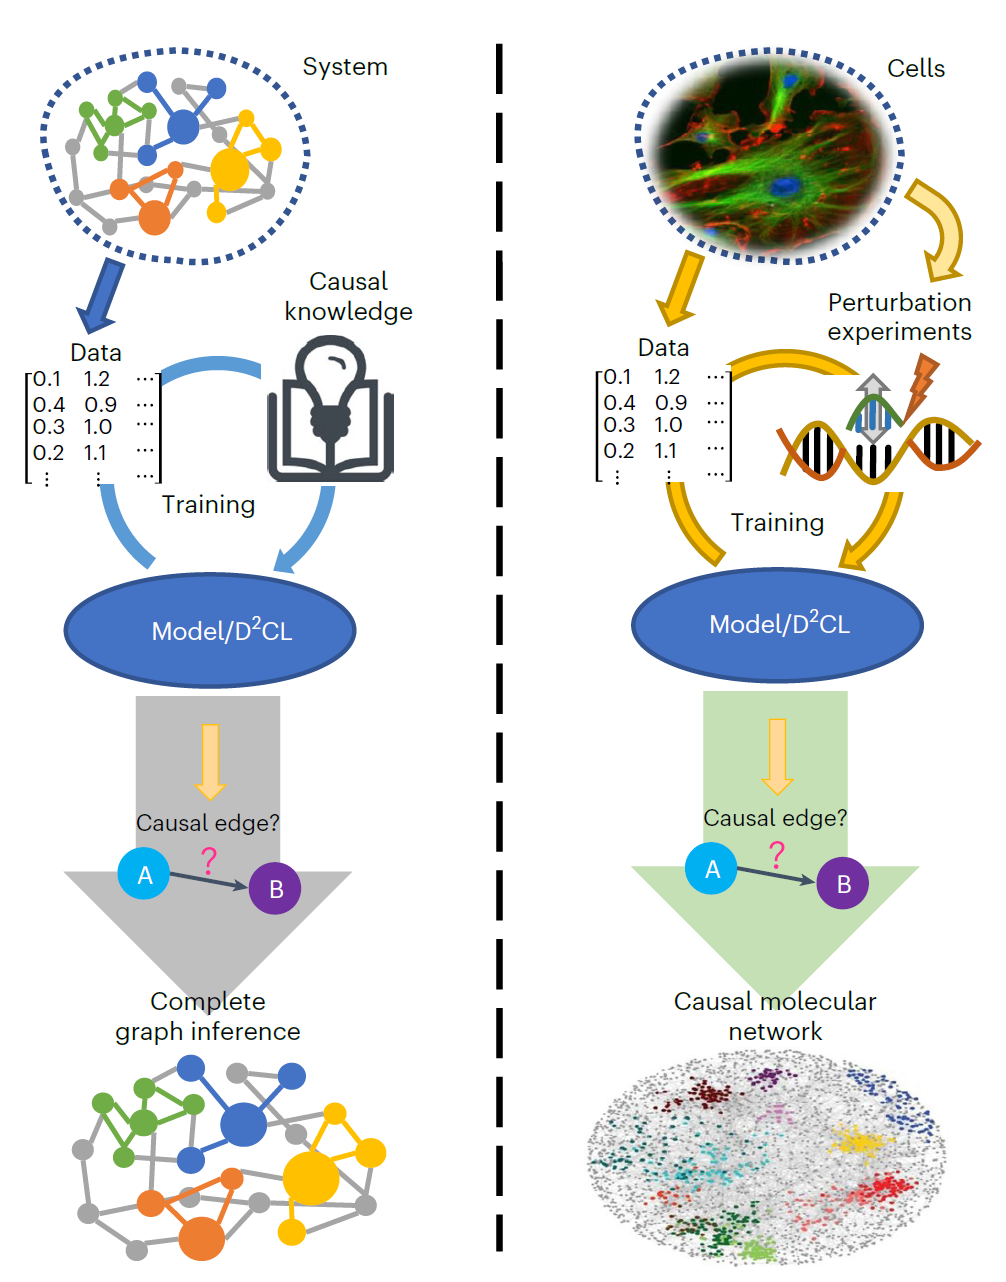
\includegraphics[height=0.6\textheight]{assets/dag-knowladge-graph.png}
        \caption{Deep learning of causal structures in high dimensions under data limitations \cite{lagemann2023deep}}
      \end{figure}
    \end{column}
  \end{columns}
\end{frame}
\begin{frame}{Judea Pearl}
  \begin{columns}[t]
    \begin{column}[t]{0.48\textwidth}
      Uno de los mayores promotores de la idea de que las redes neuronales no pueden inferir relaciones causales es Judea Pearl, quien ha argumentado que los modelos de aprendizaje profundo, como los LLMs, 
      carecen de la capacidad de representar y razonar sobre relaciones causales. Según Pearl, estos modelos se basan en correlaciones estadísticas y no pueden distinguir entre correlación y causalidad. \cite{pearl2000causality,pearl2018bookOfWhy,pearl2018theoretical}
    \end{column}
    \begin{column}[t]{0.48\textwidth}
      \begin{figure}
        \centering
        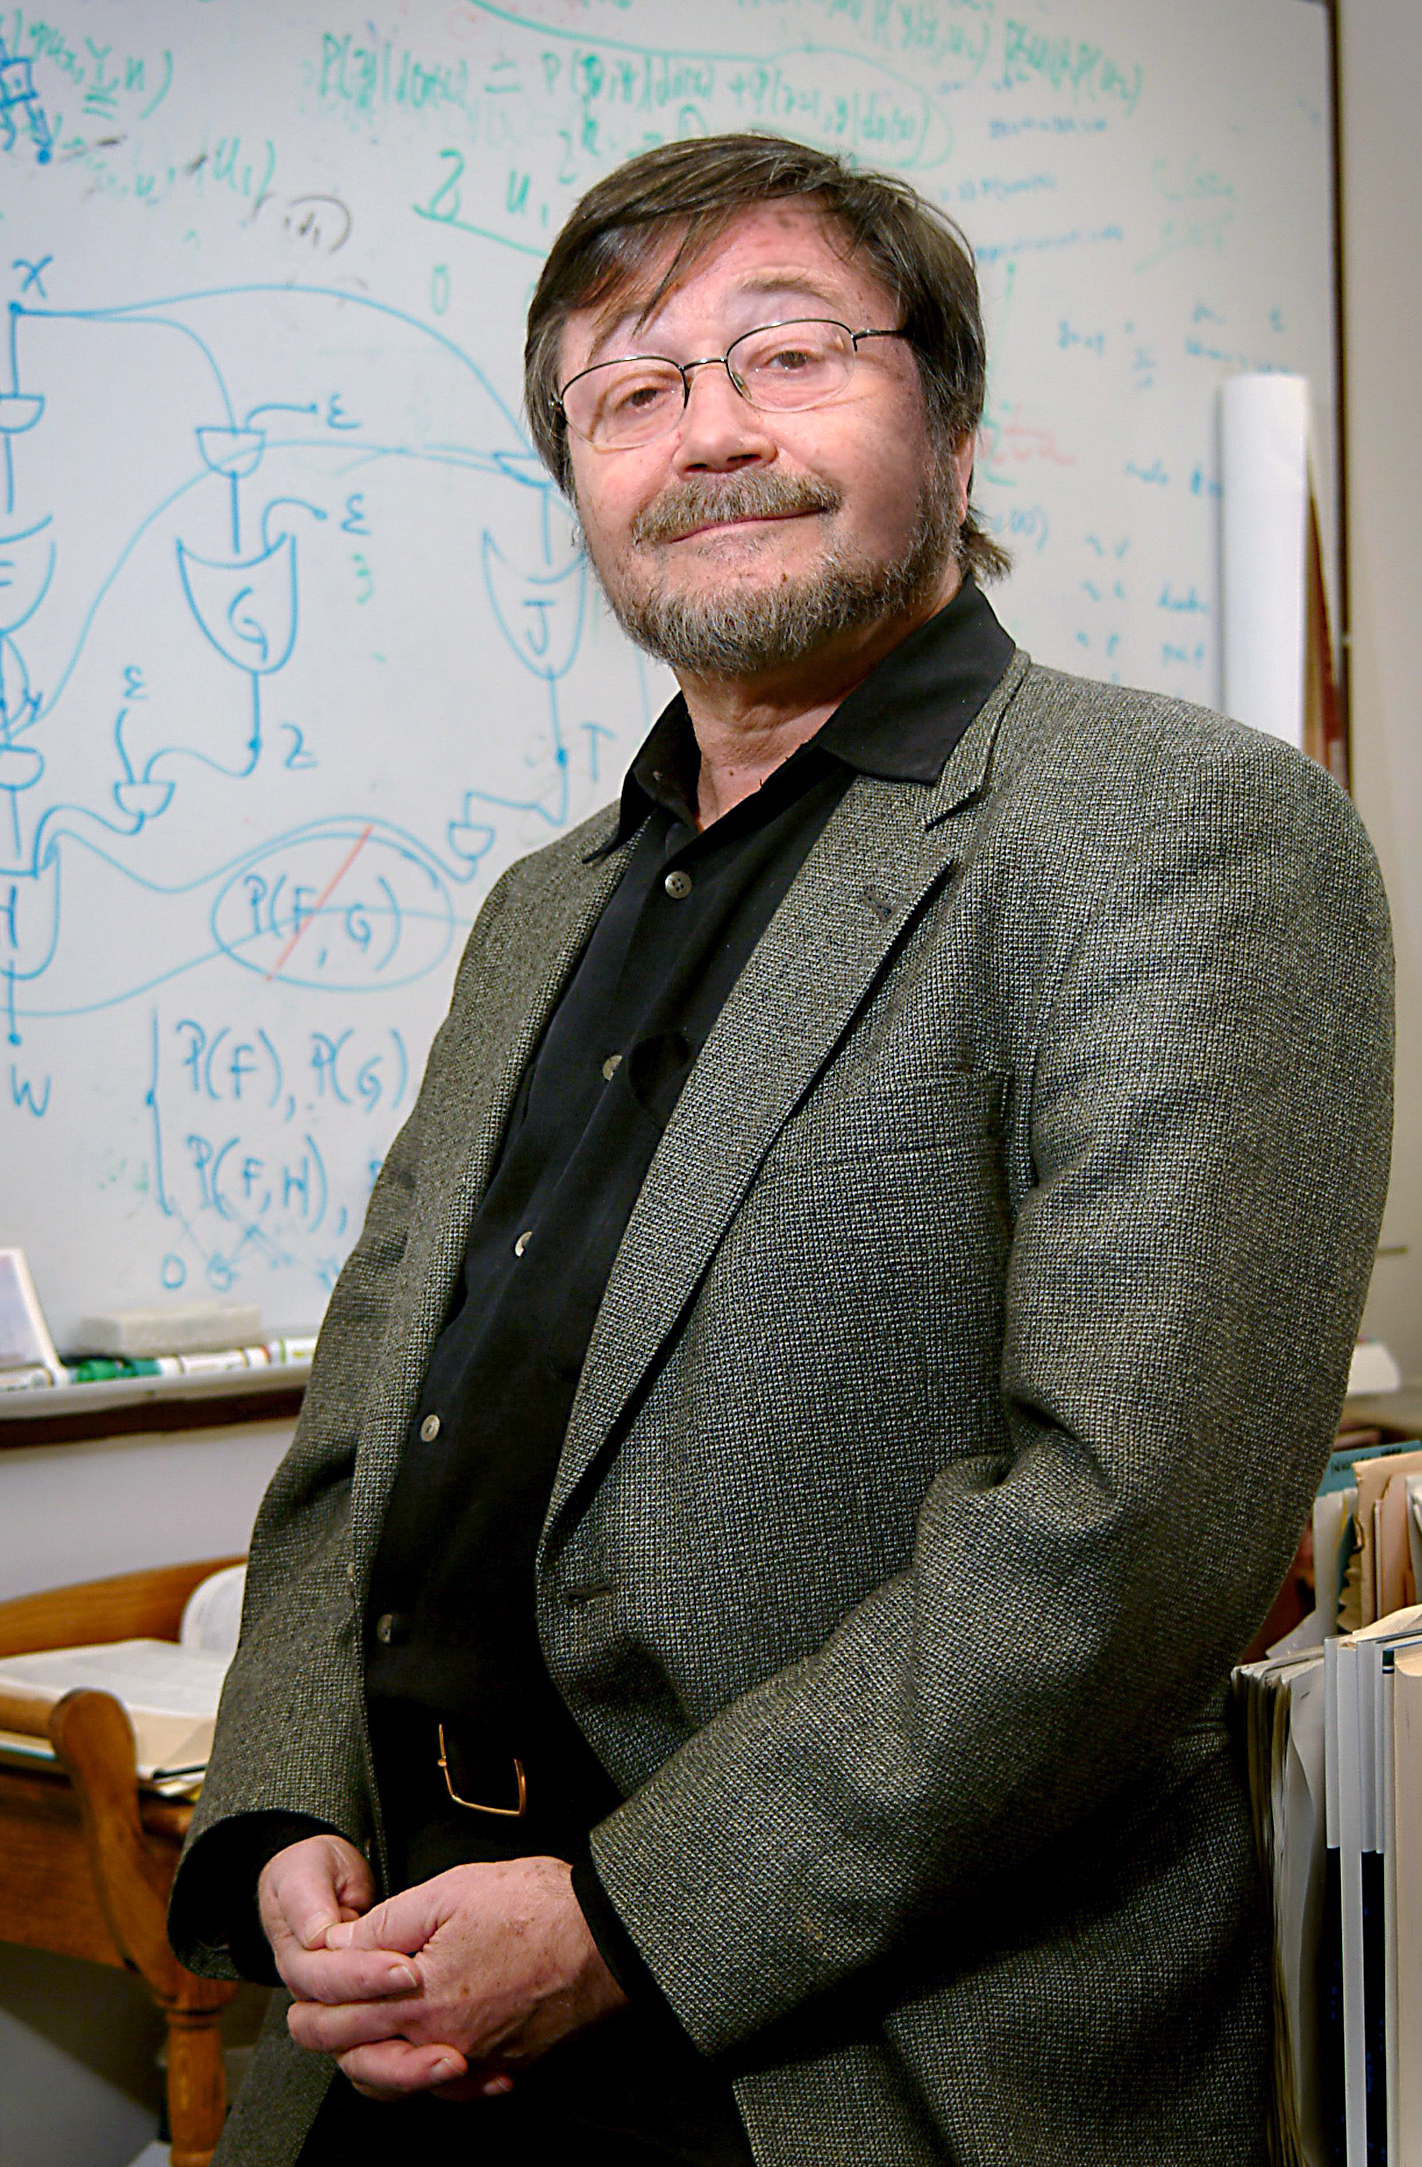
\includegraphics[width=0.6\textwidth]{assets/judea-perl.jpg}
      \end{figure}
    \end{column}
  \end{columns}
\end{frame}
\begin{frame}
  \begin{figure}
    \centering
    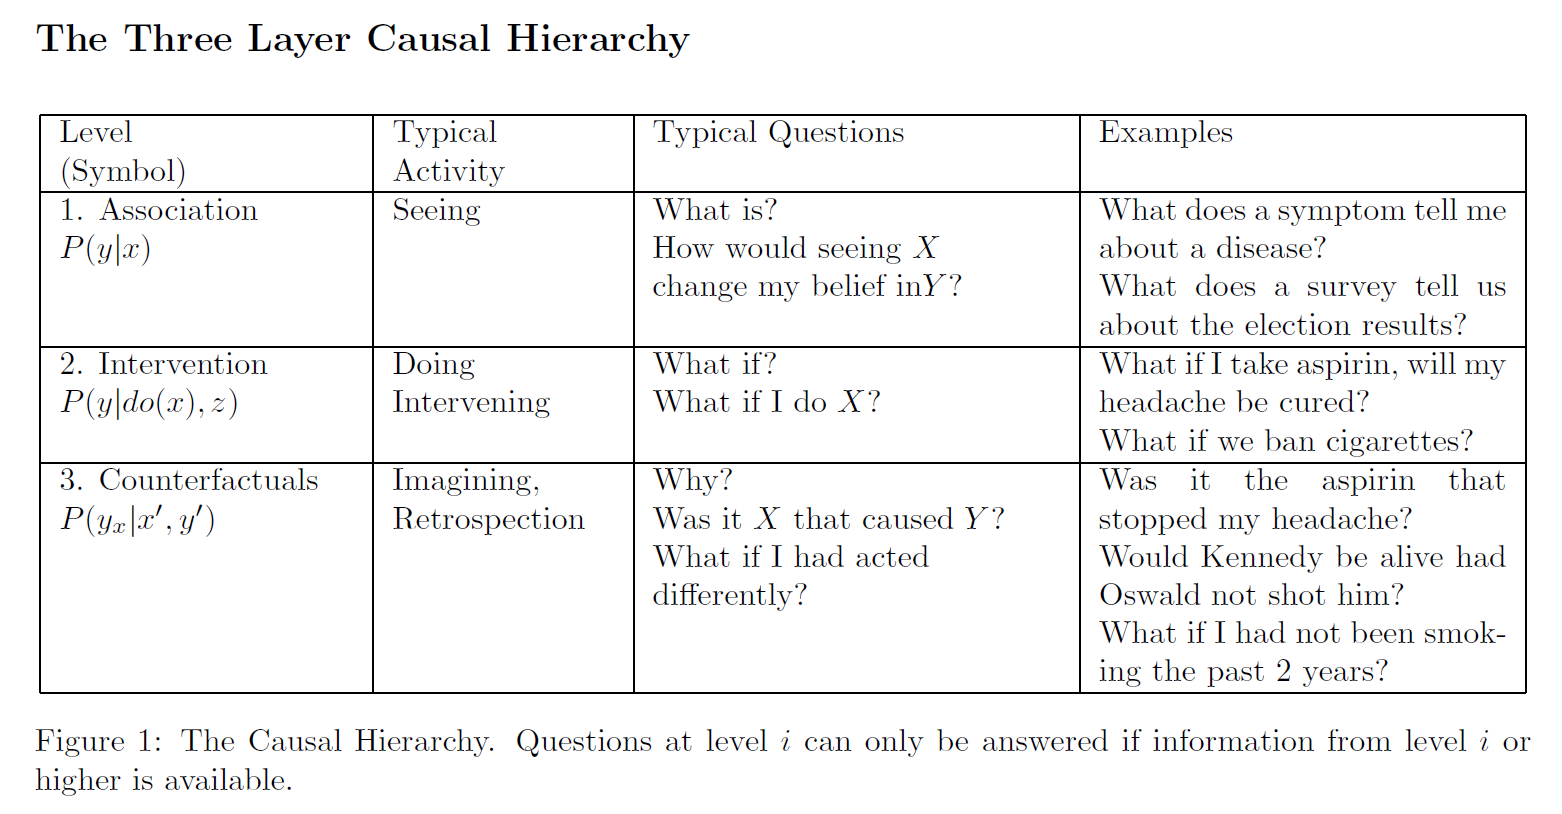
\includegraphics[height=0.4\textheight]{assets/layer-causality.png}
    \caption{La jerarquía causal de Pearl, que ilustra los diferentes niveles de inferencia causal y cómo los modelos de aprendizaje profundo se sitúan en el nivel más bajo, el de la asociación. Aunque desarrollo algunos métodos fusionando contrafácticos con teoría de grafos}
  \end{figure}
\end{frame}
\begin{frame}{Yoshua Bengio}
  \begin{columns}
    \begin{column}[t]{0.25\textwidth}
      \begin{figure}
        \centering
        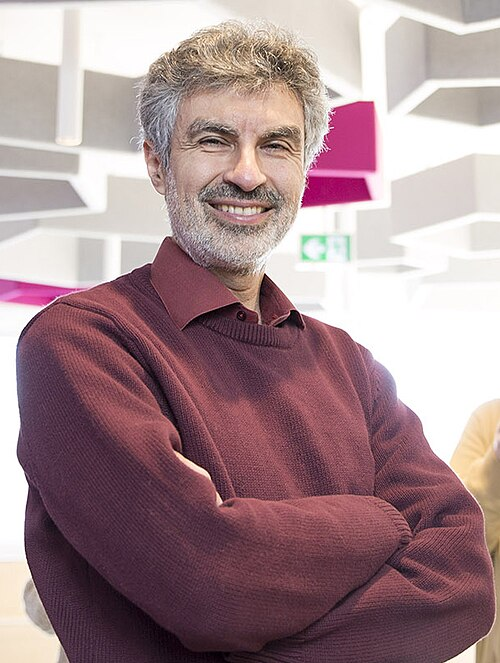
\includegraphics[width=\textwidth]{assets/Yoshua_Bengio.jpg}
      \end{figure}
    \end{column}
    \begin{column}[t]{0.6\textwidth}
      \begin{figure}
        \centering
        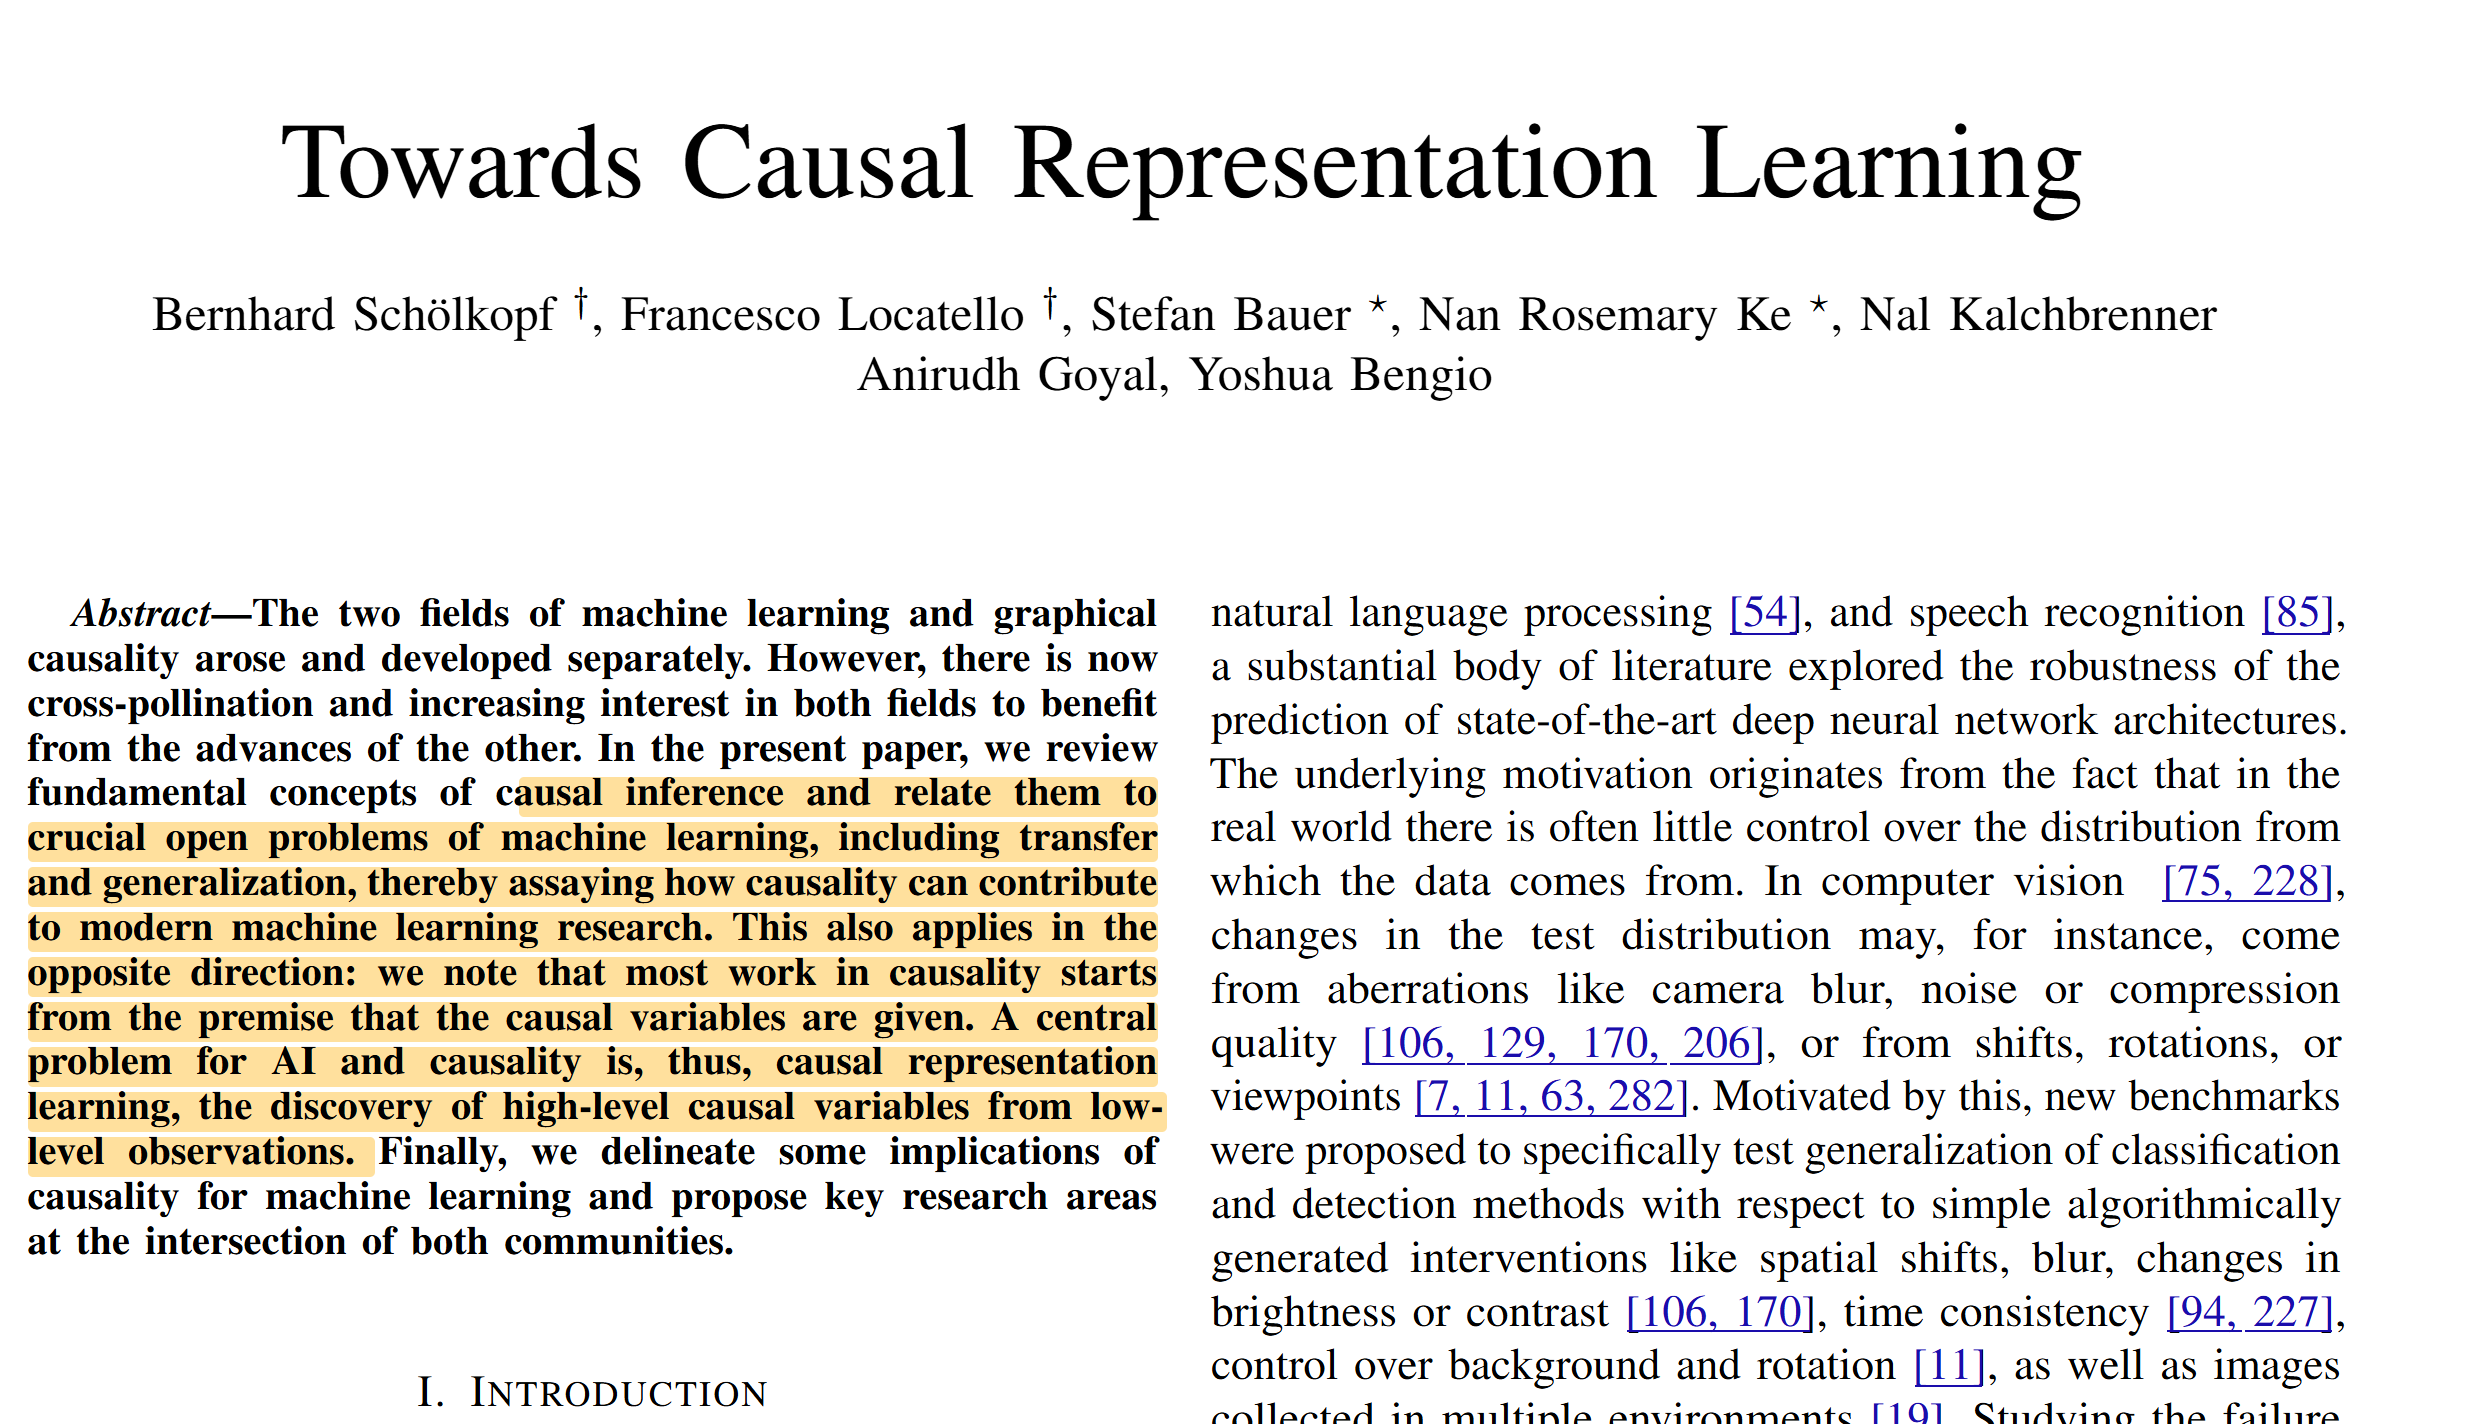
\includegraphics[width=0.6\textwidth]{assets/towards-causal.png}
        \caption{Toward causal representation learning\cite{scholkopf2021toward}}
      \end{figure}
    \end{column}
  \end{columns}
\end{frame}
\begin{frame}
  \begin{columns}
    \begin{column}{0.3\textwidth}
      Otras investigaciones se centran en modelar o encontrar inferencias causales en LLM's, modelando los datos a traves de \textit{causal embeddings}.
    \end{column}
  \begin{column}{0.7\textwidth}
    \begin{figure}
      \centering
      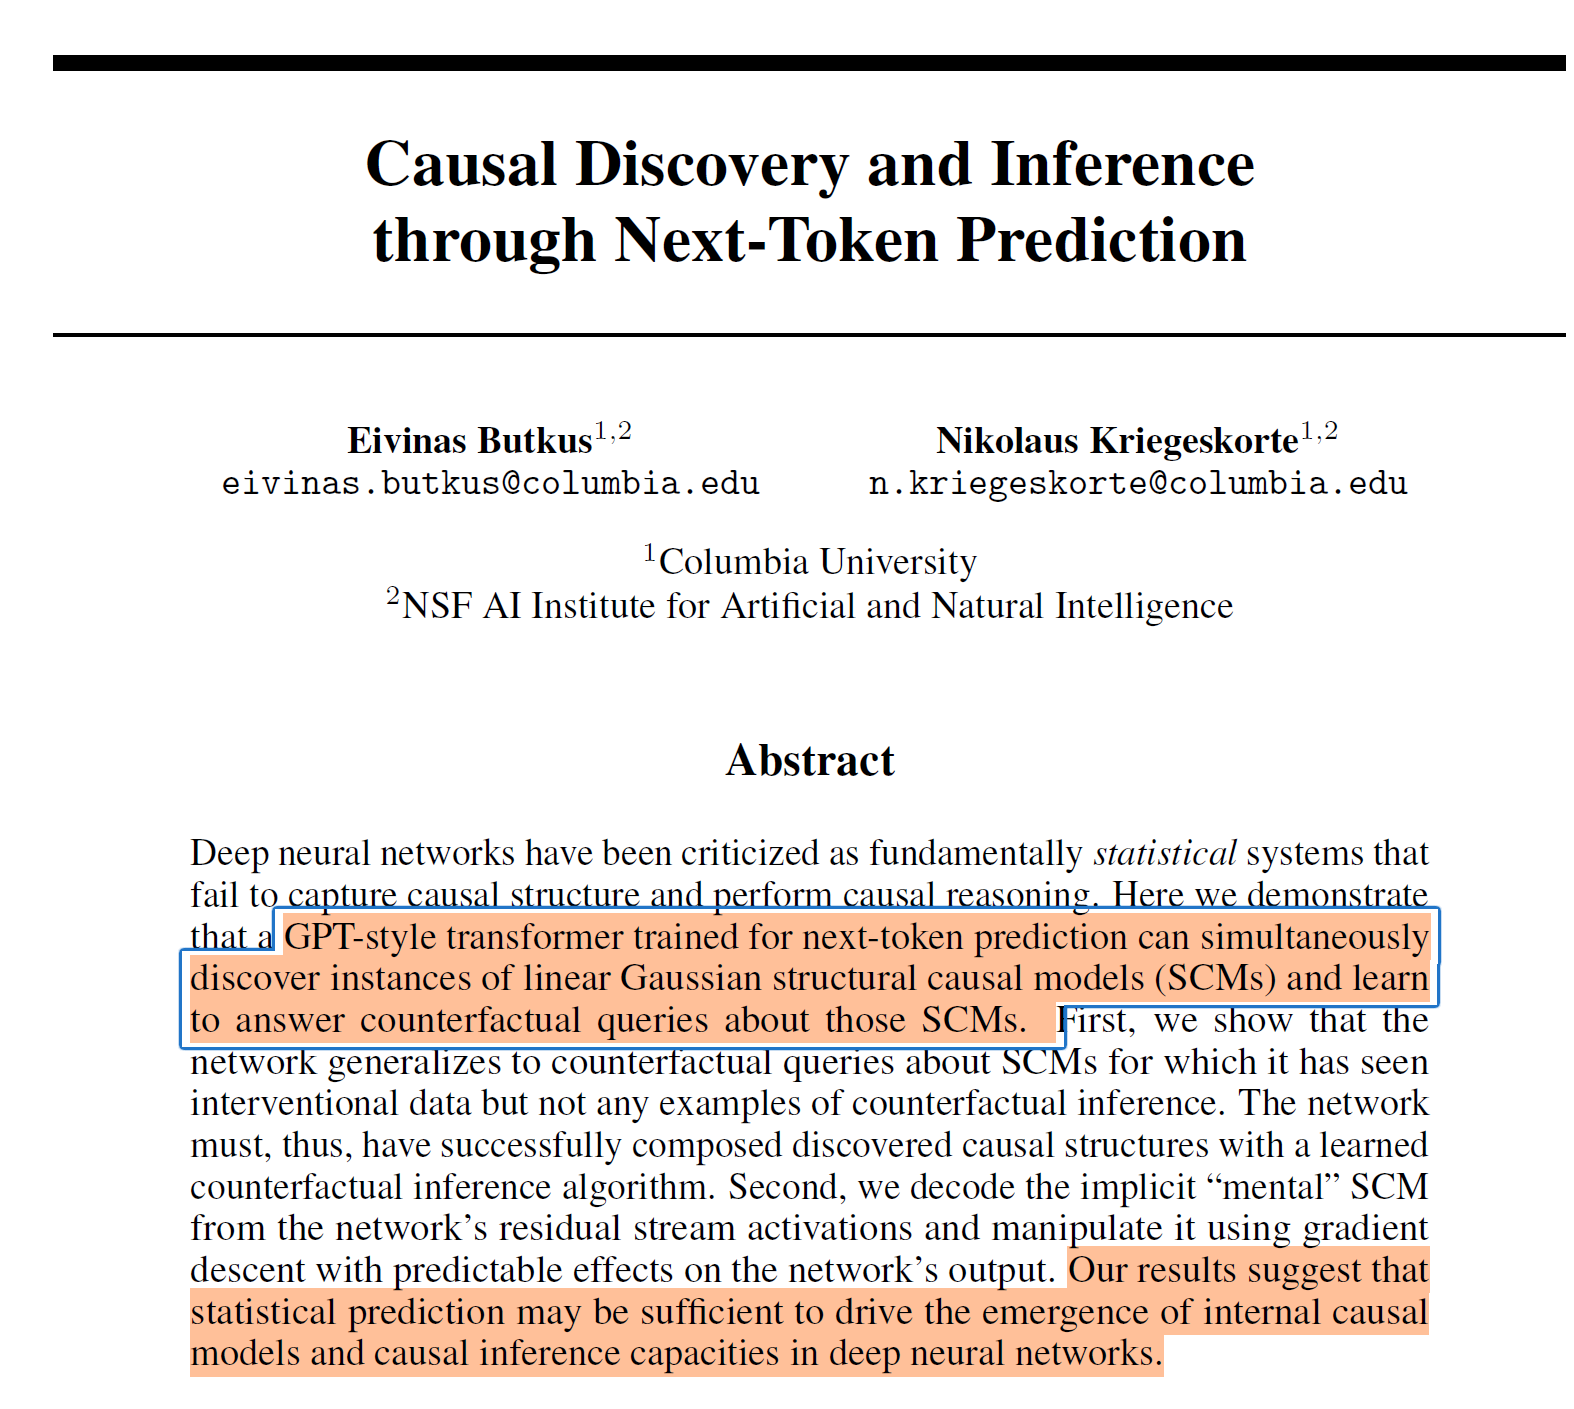
\includegraphics[width=0.7\textwidth]{assets/causal-discovery-in-llms.png}
    \end{figure}
  \end{column}
  \end{columns}
\end{frame}
\begin{frame}{Estado del Arte}
  Existe un programa llamado \textit{Topological Deep Learning} (Topological Deep Learning is the New Frontier for Relational Learning)\cite{papamarkou2024position} que explora invariantes geométricas y topológicas en los modelos de redes neuronales. La idea central es encontrar diferentes maneras de obtener resultados con aprendizaje profundo y datos relacionales. 
  Para entender y lograr capturar las relaciones subyacentes a los datos. 
  \begin{figure}
    \centering
    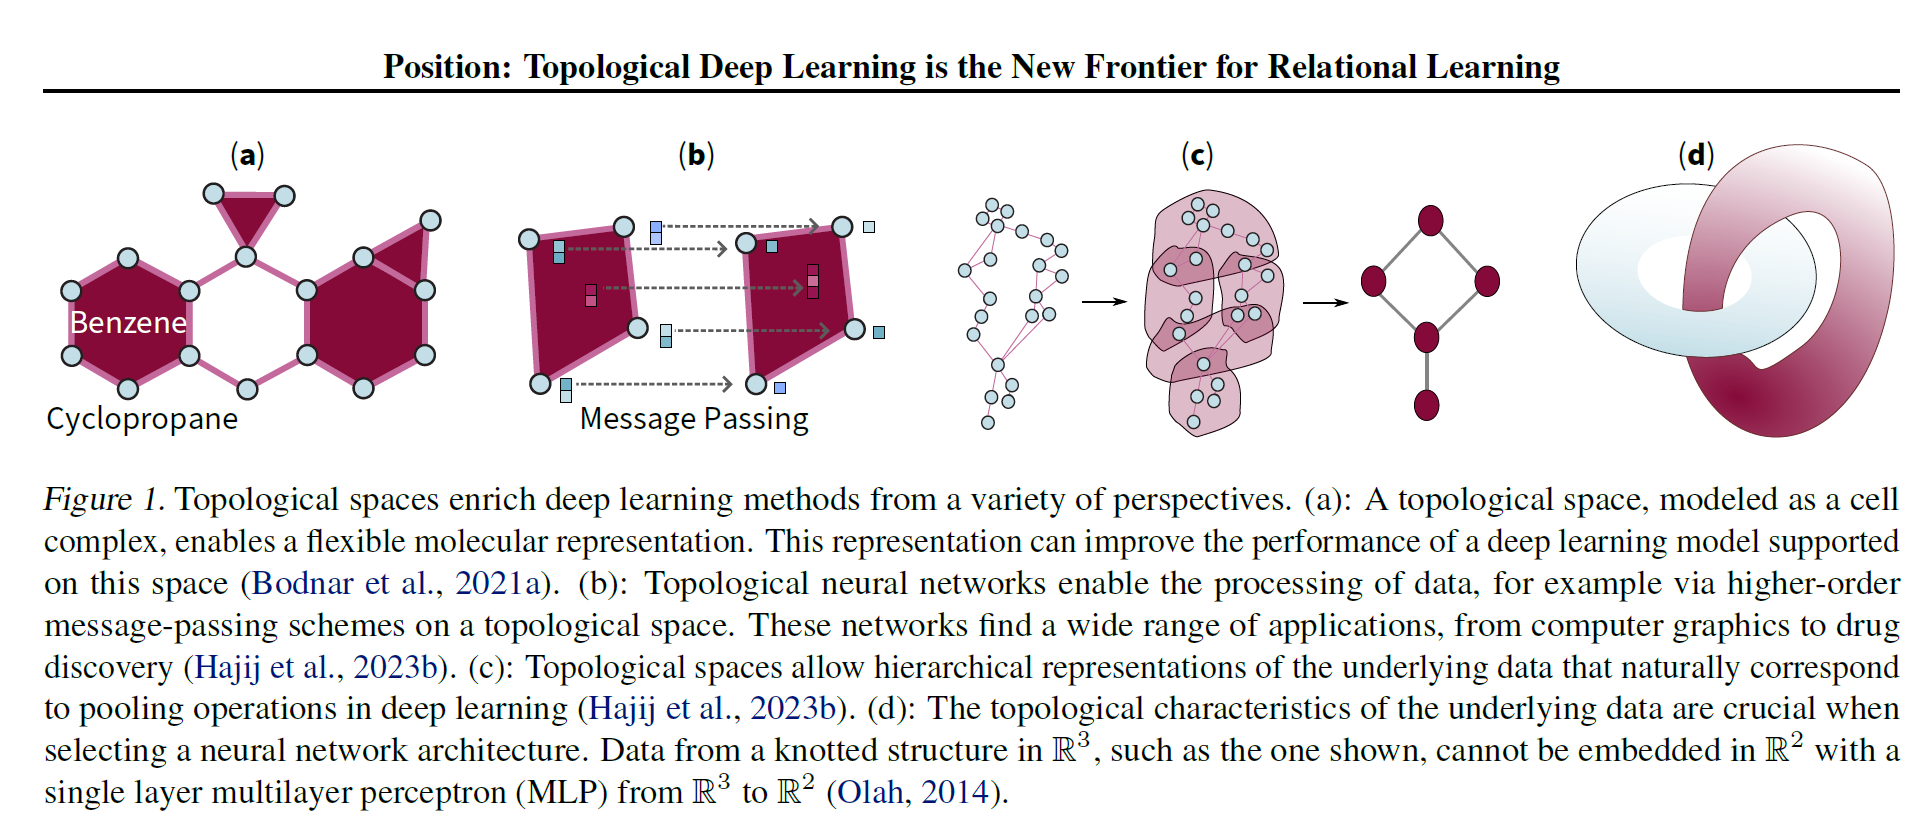
\includegraphics[width=0.5\textwidth]{assets/topological-relationship.png}
    \caption{Ejemplo en células.\cite{papamarkou2024position}}
  \end{figure}
\end{frame}
\begin{frame}
    \begin{itemize}
    \item La topología del espacio de datos subyacente determina qué arquitecturas de redes neuronales son viables
    \item Los dominios topológicos permiten modelar datos que contienen interacciones de múltiples niveles (relaciones de orden superior / \textbf{complejidad})
    \item El aprendizaje profundo topológico captura regularidades propias de las variedades (\textbf{explicabilidad} en LLM's). 
    \item Detecta las equivarianzas topológicas presentes en los datos (\textbf{inferencias causales}).
    \item Integra características topológicas inherentes a datos relacionales. (\textbf{interpretabilidad}). 
  \end{itemize}
\end{frame}
\subsection{Ejemplos en la Ciencia}
\begin{frame}{COSMIC Cancer Database }
  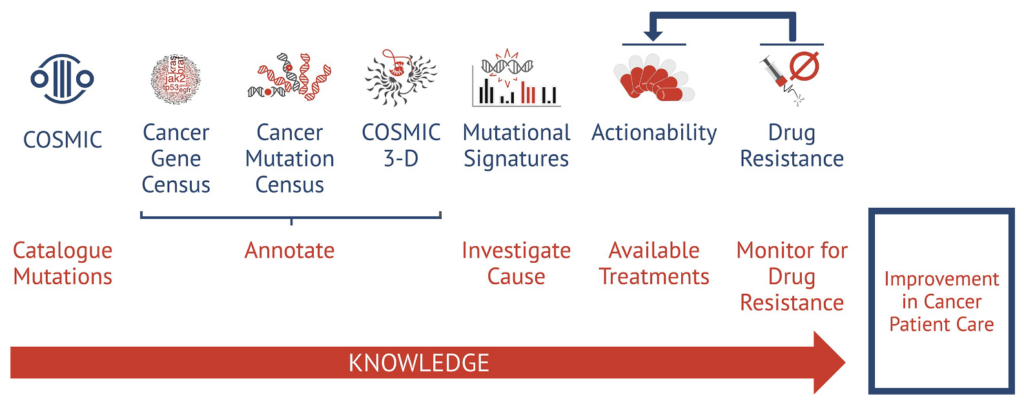
\includegraphics[width=\textwidth]{assets/cancer-database.png}
\end{frame}
\begin{frame}{Relaciones en la Ciencias}
  COSMIC es una base de datos de mutaciones genéticas en cáncer, que se ha utilizado para entrenar modelos de redes neuronales con el fin de identificar genes impulsores del cáncer. \\
  Artículos recientes: 
  \begin{itemize}
    \item Trans-Driver: A Deep Learning Approach for Cancer Driver Gene Discovery With Multi-Omics Data \cite{yang2025trans}
    \item Explainable Multilayer \textbf{Graph Neural Network} for cancer gene prediction \cite{chatzianastasis2023explainable}
    \item DGMP: Identifying Cancer Driver Genes by Jointing DGCN and MLP from Multi-omics Genomic Data (\textbf{Directed graph convolutional network}, Multilayer perceptron) \cite{zhang2022dgmp}
  \end{itemize}
\end{frame}
\subsection{Diferentes Arquitecturas}
\begin{frame}{Gráficas de Conocimiento}
  \begin{figure}
    \centering
    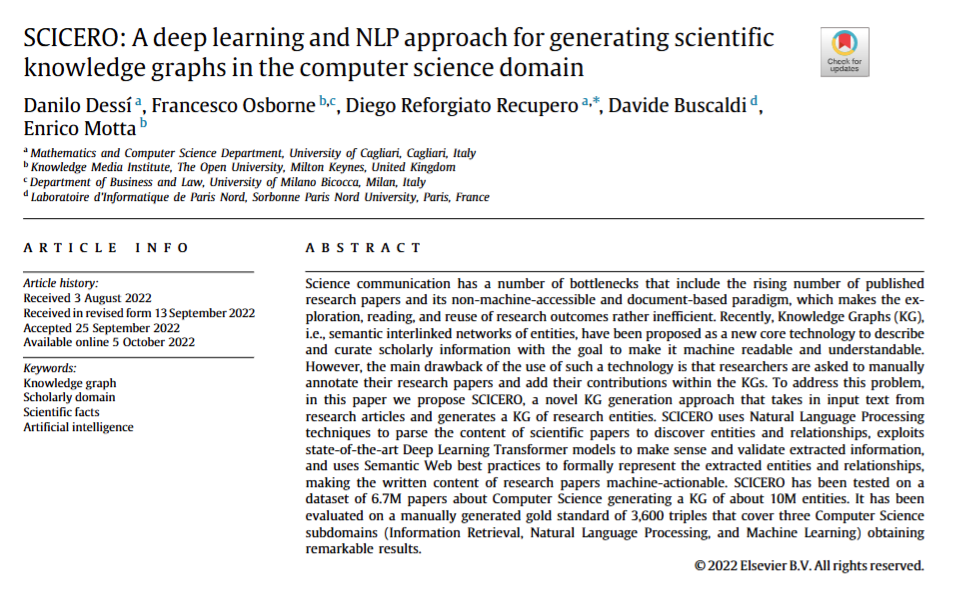
\includegraphics[width=0.6\textwidth]{assets/SCICERO.png}
    \caption{Ejemplo de la construcción de un grafo de conocimiento científico, que representa relaciones entre conceptos, descubrimientos y publicaciones en un campo específico.\cite{dessi2022scicero}}
  \end{figure}
\end{frame}

\begin{frame}{Graph Neural Networks}
  Unmasking Hidden Fraud Patterns: An Explainable Graph Attention Network Approach for Highly Imbalanced Financial Datasets(Oguntola, 2026)
  \begin{figure}
    \centering
    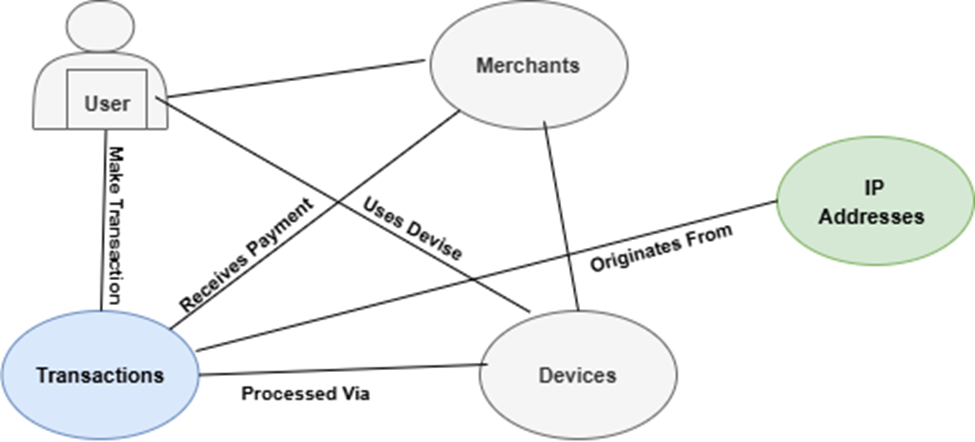
\includegraphics[width=0.6\textwidth]{assets/transactions-relationships.png}
    \caption{Ejemplo de una red neuronal gráfica, que detecta fraudes fiscales la ventaja comparativa hace que tenga un desempeño superior a otras arquitecturas de redes neuronales además de permitirnos 
    analizar relaciones complejas entre entidades.\cite{oguntola2026unmasking}}
  \end{figure}
\end{frame}
\begin{frame}{Manifolds}
  \begin{columns}[t]
    \begin{column}[t]{0.48\textwidth}
      \small
      Variedades(Espacios curvos multi dimensionales $\mathds{R}^n$). Este tipo de aproximaciones son el trabajo de ingeniería inversa con respecto al ordenamiento de los datos. A comparación de las arquitecturas tipo DAG, esta metodología se vuelve más top-down, ya que se enfoca en la representación de los datos y no en la construcción de una arquitectura específica.
      Se apoya en la idea de que~``Las distancias geodésicas en las variedades de representación de los LLM son significativas'' \cite{modell2025origins}.
    \end{column}
    \begin{column}[t]{0.48\textwidth}
      \begin{figure}
      \centering
      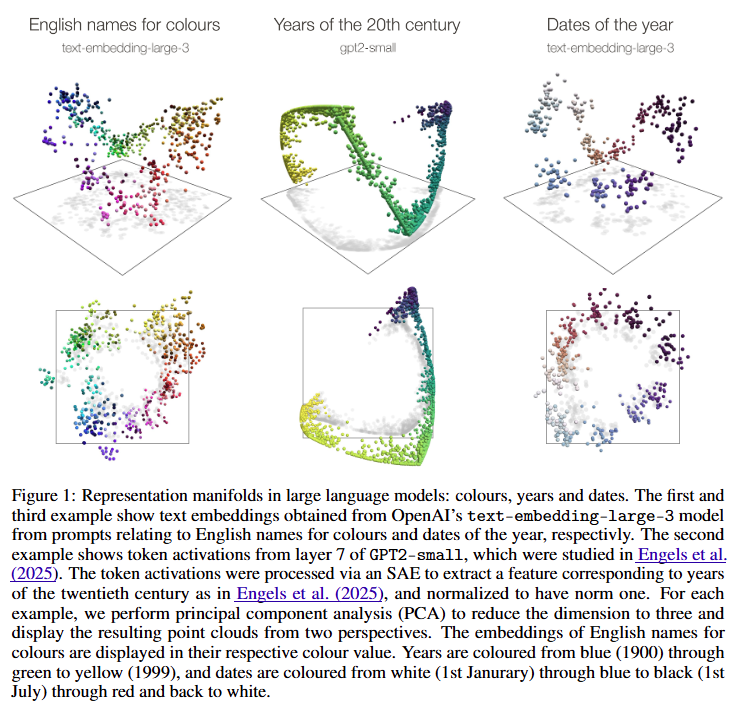
\includegraphics[width=0.8\textwidth]{assets/lrh-manifold.png}
      \end{figure}
    \end{column}
    \end{columns}
\end{frame}

\begin{frame}[allowframebreaks]{References}
  \bibliographystyle{unsrt}
  \bibliography{reference.bib}
\end{frame}

\end{document}